\documentclass[titlepage]{jsarticle}
\usepackage[dvipdfmx]{graphicx}
\usepackage{bm}
\usepackage{amsmath}
\usepackage{amssymb}
\usepackage{amsfonts}
\usepackage{here}
\usepackage{comment}
\usepackage{listings}
\lstset{
    basicstyle={\ttfamily},
    identifierstyle={\small},
    commentstyle={\smallitshape},
    keywordstyle={\small\bfseries},
    ndkeywordstyle={\small},
    stringstyle={\small\ttfamily},
    frame={tb},
    breaklines=true,
    columns=[l]{fullflexible},
    numbers=left,
    xrightmargin=0zw,
    xleftmargin=3zw,
    numberstyle={\scriptsize},
    stepnumber=1,
    numbersep=1zw,
    lineskip=-0.5ex,
    keepspaces=true,
    language=c
}
\renewcommand{\lstlistingname}{ソースコード}
\makeatletter
\newcommand{\figcaption}[1]{\def\@captype{figure}\caption{#1}}
\newcommand{\tblcaption}[1]{\def\@captype{table}\caption{#1}}
\makeatother




\begin{document}
\title{数値解析レポートNo.3}
\author{40番 矢野 敦大}
\date{}
\maketitle

\section{指数近似}
	多項式以外の一般的な近似方法の1つに指数近似
	\begin{equation}
		y = a_0e^{a_1x}
		\label{equ:1}
	\end{equation}
	がある。
	ここでは以下のデータを指数近似してグラフを示す。
	
	(x, y) = (1.5, 8.96), (2.0, 14.78), (2.5, 24.36), (3.0, 40.17)\\
	式(\ref{equ:1})で両辺の対数を取ると、
	\begin{equation}
		\ln y = \ln a_0 + a_1x
		\label{equ:2}
	\end{equation}
	となり、一次近似を行うことができる。
	線形近似のプログラムを指数近似に対応させたプログラムをソースコード\ref{src:ichiji}に示す。今回は最小二乗法を利用し、
	線形近似を実現する。
	関数exp$\_$approxmationで配列a[0],a[1]に格納される値はそれぞれ、式(\ref{equ:2})の$a_0,a_1$に対応している。	
	線形近似の一般的な形は、$y = a_0 + a_1 x$なので、7,18行目で今回の指数近似の形に項を合わせている。
\begin{lstlisting}[caption=作成した指数近似を行うプログラム\cite{wiki},label=src:ichiji]
void exp_approxmation(double *a, double* X, double* Y) {
	
	int i;
	double x = 0, y = 0, xx = 0, xy = 0, n = DATANUM;

	for (i = 0; i < n; i++) {
		Y[i] = log(Y[i]);
	}
	for (i = 0; i < n; i++) {
		x += X[i];
		y += Y[i];
		xx += X[i] * X[i];
		xy += X[i] * Y[i];
	}
	a[0] = (y * xx - x * xy) / (n * xx - x * x);
	a[1] = (n * xy - x * y) / (n * xx - x * x);

	a[0] = exp(a[0]);
	return;
}
\end{lstlisting}
	このプログラムにより今回のデータを指数近似した結果、$a_0\approx 1.99911,a_0\approx 1.00014$となった。
	これらの値を利用し$y$をグラフ化した様子を図\ref{fig:1}に示す。きれいな指数関数の形になっていることがわかる。

	\begin{figure}[]
		\centering
		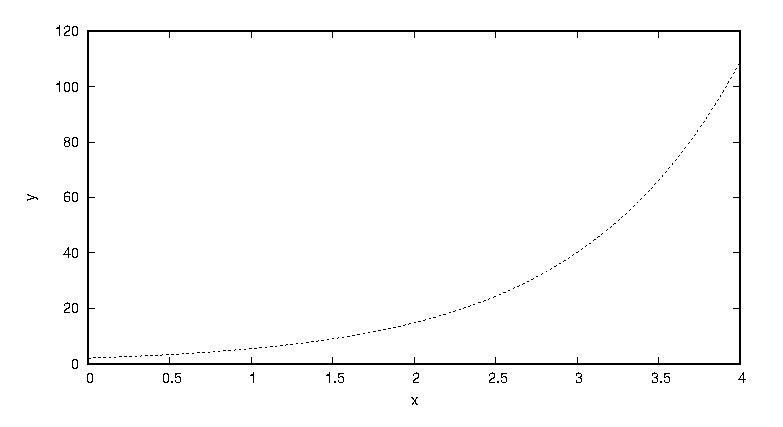
\includegraphics[height=7cm]{1/res.eps}
		\caption{指数近似により求めた$y$のグラフ}
		\label{fig:1}
	\end{figure}

\section{これまでの相互評価課題について}
	\subsection{良いと思うところ、参考になったところ}
		私は今まで部活等で他人のコードを読むことはあったが、なんとなく流し読みする程度だった。今回初めて相互評価を
		するために、他人のコードをじっくり読み込む体験をした。他人のコードを見ていると、インデントの大きさや、変数名のつけ方、	
		コメントの量など人それぞれのスタイルが見られ、自分のコーディングの改善につながった。
		自分のコードの悪いところも指摘してもらうことができたのが良かった。
		将来業務で他人とプログラムを共有するような仕事をするようになった時にこの経験がいきると思った。来年度以降の
		数値解析の授業でも継続したほうが良いと思う。


	\subsection{改善すべきところ、改善案、バグ報告}
		相互評価の改善案だが、他人からのフィードバックが次の課題の提出後となっていたため、フィードバックの内容が
		次の課題に反映できないことがあったので、結果の返却を早めに行ってほしいと思った。

	\subsection{疑問・感想}
		相互評価についての疑問は特にない。感想は2.1節と被る部分もあるが、他人のコードを読むことと、他人からの
		フィードバックを通して自分のプログラミング能力を向上させることができたのでとても良かった。
		

\section{3種の数値積分の比較}
	今回は台形公式、シンプソン公式、ロンバーク積分の3種の数値積分の方法を(1)分割数と誤差、(2)計算量の二つの観点から
	比較を行う。
	
	これらの三つの手法で定積分を行った結果を比較するプログラムをソースコード\ref{src:2}に示す。
\begin{lstlisting}[caption=作成した数値積分を行うプログラム, label=src:2]
double trapezoid(double a, double b, int n) {

	double sum = 0, h = (b - a) / n, x = a;
	int i;
	for (i = 1; i < n; i++) {
		x += h;
		sum += f(x);
	}
	sum += (f(a) + f(b)) / 2;
	sum *= h;
	return sum;
}

double simpson(double a, double b, double n) {

	int i;
	double sum = 0, h = (b - a) / (2 * n), x = a, mid;
	
	for (i = 1; i <= n; i++) {
		mid = x + h;
		sum += (4 * f(mid) + f(x) + f(x + h)) * h / 3;
		x += h * 2;
	}
	return sum;
}

double romberg(double a, double b, int n) {
	
	double tmp;
	double r[n + 1][n + 1];
	int i, j, k;

	r[1][1] = (b - a) / 2 * (f(a) + f(b));

	for (k = 2; k <= n; k++) {
		tmp = 0;
		for (i = 1; i <= pow(2, k - 2); i++) {
			tmp = tmp + f(a + (2 * i - 1) * (b - a) / pow(2, k - 1));
		}
		r[k][1] = (r[k - 1][1] + (b - a) / pow(2, k - 2) * tmp) / 2;
	}

	for (k = 2; k <= n; k++) {
		for (j = 2; j <= k; j++) {
			r[k][j] = r[k][j - 1] + (r[k][j - 1] - r[k - 1][j - 1]) / (pow(4, j - 1) - 1);
		}
	}
	return r[n][n];
}
\end{lstlisting}
	\subsection{分割数と誤差}
		今回はこのプログラムを使って、$\displaystyle \int^3_1 e^x dx$,$\displaystyle \int^2_1 x^2\ln (x+1)dx$の値を求め、
		誤差を比較しようと思う。真の値はそれぞれ$\displaystyle \int^3_1 e^x dx \approx 17.367255$,
		$\displaystyle \int^2_1 x^2\ln (x+1)dx \approx 2.2226$である。図\ref{fig:res1},\ref{fig:res2}は分割数nと
		真値との誤差を表したグラフである。これらのグラフを見ると、ロンバーグ法、台形公式、シンプソン公式の順に収束が早いことがわかる。
		特にロンバーグ法は、分割数が2程度でも非常に精度の高い解が得られることがわかる。
		\begin{figure}[H]
			\centering
			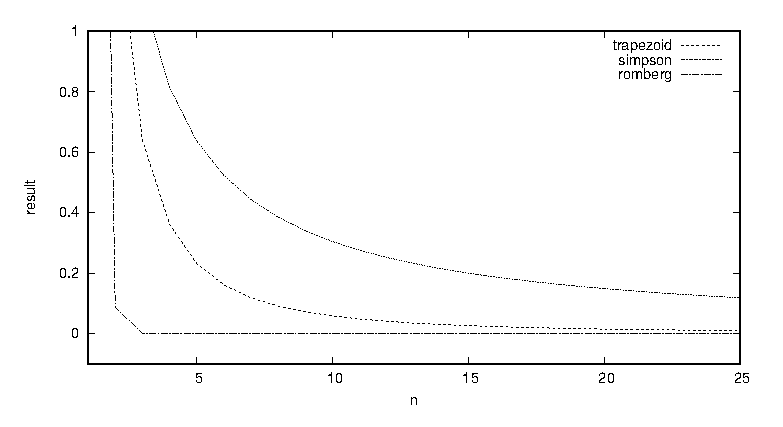
\includegraphics[height=7cm]{2/res1.eps}
			\caption{3手法で$\displaystyle \int^3_1 e^x dx$を積分した結果の比較}
			\label{fig:res1}
		\end{figure}

		\begin{figure}[]
			\centering
			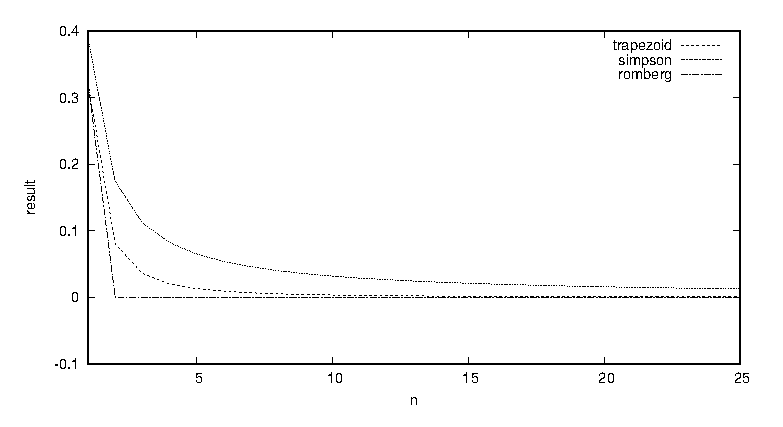
\includegraphics[height=7cm]{2/res.eps}
			\caption{3手法で$\displaystyle \int^2_1 x^2\ln (x+1)dx$を積分した結果の比較}
			\label{fig:res2}
		\end{figure}


	\subsection{計算量}
		台形公式、シンプソン公式はプログラムも一重ループであることから分かるように、計算量は分割数をnとすると
		$O(n)$である。
		ロンバーク積分の分割数は$2^n$となる。ソースコード\ref{src:2}の35,37行目のfor文から、$O(2^n)$と推測できる。
		ロンバーグ積分は
		少ない分割数でも精度の良い解を得ることができるので、分割数はあまり増やさないほうが良い。。


\begin{thebibliography}{99}
        \bibitem{wiki} ウィキペディア-最小二乗法, \\
            "https://ja.wikipedia.org/wiki/最小二乗法"
\end{thebibliography}       
\end{document}




























